\documentclass[preview]{standalone}
% \documentclass{scrartcl}
\usepackage{tikz}
\begin{document}
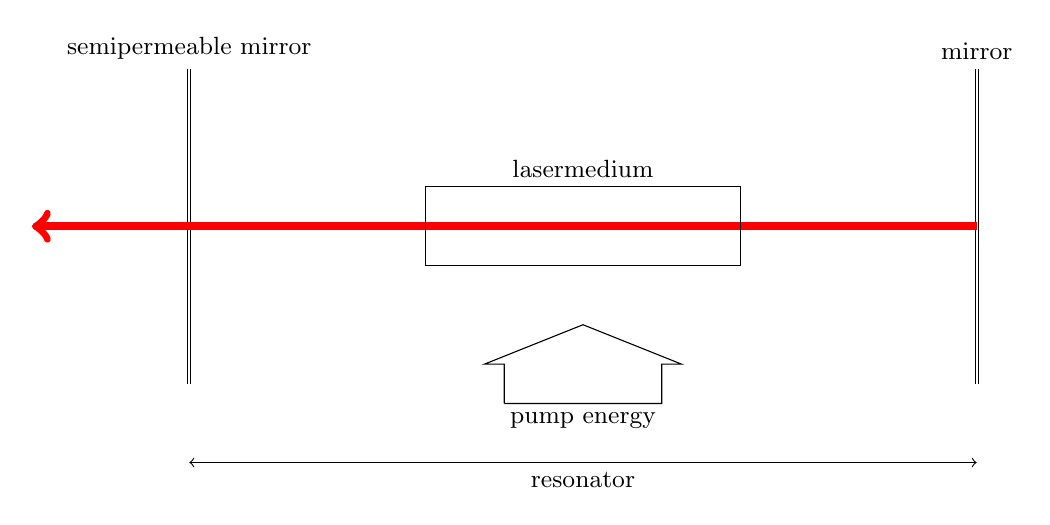
\begin{tikzpicture}

\coordinate(left) at (0,0);
\coordinate(right) at (10,0);

\draw[double] (left) to ++ (0,4) node[above]{\small semipermeable mirror};
\draw[double] (right) to ++ (0,4) node[above]{\small mirror};

\draw[line width=3pt,red,->] (right) ++ (0,2) to ++ (-12,0);

\draw (left) ++ (3,1.5)
    to ++ (0,1)
    to node[above]{\small lasermedium} ++ (4,0)
    to ++ (0,-1)
    to ++ (-4,0) circle;

\draw[<->] (left) ++ (0,-1) to node[below]{\small resonator} ++ (10,0);

\draw
  (4,-0.25)
  to node[below]{\small pump energy} ++ (2,0)
  to ++ (0,0.5)
  to ++ (0.25,0)
  to ++ (-1.25,+0.5)
  to ++ (-1.25,-0.5)
  to ++ (0.25,0)
  to ++ (0,-0.5)
  circle;



\end{tikzpicture}

% \begin{tikzpicture}


% \usetikzlibrary{decorations.pathmorphing}

% \tikzset{%
%   photon/.style   = {red,decorate,decoration={snake},->},
%   electron/.style = {blue,dashed,->},
%   border/.style   = {thick},
% }

% % \coordinate(ind)  at (10,0); % Induced Emission
% % \draw[border]   (ind) ++ (0,1) to node[above]{Induced emission} ++ (2,0);
% % \draw[border]   (ind) to ++ (2,0);
% % \draw[electron] (ind) ++ (1,1) to ++ (0,-1);
% % \draw[photon]   (ind) ++ (0,0.75) to ++ (1,0);
% % \draw[photon]   (ind) ++ (1,0.75) to ++ (1,0);
% % \draw[photon]   (ind) ++ (1,0.25) to ++ (1,0);


% \end{tikzpicture}
\end{document}
